\subsection{Tabele}

Wszystkie tabele są tworzone przez 13 skryptów \texttt{SQL}:
\begin{itemize}
	\item \href{run:Sources/SQL/1. Tabele/001_Utworzenie_tabeli_z_miastami.sql}{Utworzenie tabeli z miastami}
	\item \href{run:Sources/SQL/1. Tabele/002_Utworzenie_tabeli_z_dzielnicami.sql}{Utworzenie tabeli z dzielnicami}
	\item \href{run:Sources/SQL/1. Tabele/003_Utworzenie_relacji_pomiedzy_miastami_a_dzielnicami.sql}{Utworzenie relacji pomiedzy miastami a dzielnicami}
	\item \href{run:Sources/SQL/1. Tabele/004_Utworzenie_tabeli_z_kategoriami.sql}{Utworzenie tabeli z kategoriami}
	\item \href{run:Sources/SQL/1. Tabele/005_Utworzenie_tabeli_z_obiektami.sql}{Utworzenie tabeli z obiektami}
	\item \href{run:Sources/SQL/1. Tabele/006_Utworzenie_relacji_pomiedzy_dzielnicami_a_obiektami.sql}{Utworzenie relacji pomiedzy dzielnicami a obiektami}
	\item \href{run:Sources/SQL/1. Tabele/007_Utworzenie_relacji_pomiedzy_kategoriami_a_obiektami.sql}{Utworzenie relacji pomiedzy kategoriami a obiektami}
	\item \href{run:Sources/SQL/1. Tabele/008_Utworzenie_tabeli_z_uzytkownikami.sql}{Utworzenie tabeli z uzytkownikami}
	\item \href{run:Sources/SQL/1. Tabele/009_Utworzenie_tabeli_z_najmami.sql}{Utworzenie tabeli z najmami}
	\item \href{run:Sources/SQL/1. Tabele/010_Utworzenie_indeksu_unikatowego_w_tabeli_z_najemcami.sql}{Utworzenie indeksu unikatowego w tabeli z najmami}
	\item \href{run:Sources/SQL/1. Tabele/011_Utworzenie_relacji_pomiedzy_uzytkownikami_a_najmami.sql}{Utworzenie relacji pomiedzy uzytkownikami a najmami}
	\item \href{run:Sources/SQL/1. Tabele/012_Utworzenie_relacji_pomiedzy_obiektami_a_najmami.sql}{Utworzenie relacji pomiedzy obiektami a najmami}
	\item \href{run:Sources/SQL/1. Tabele/013_Utworzenie_indeksu_unikatowego_w_tabeli_z_uzytkownikami.sql}{Utworzenie indeksu unikatowego w tabeli z uzytkownikami}
\end{itemize}

Tworzenie relacji pomiędzy tabelami oraz indeksów zostało oddzielone od operacji tworzenia poszczególnych tabel - celem tego działania jest lepsza organizacja skryptów. Dodatkowo oddzielając te operacje, w przypadku wystąpienia jakiegoś błędu jesteśmy w stanie określić co i gdzie się "wysypało".

Ze względu na to aby nie zajmować zbyt dużo miejsca, poniżej zostaną przedstawione tylko najważniejsze z powyższych skryptów.

\subsubsection{Utworzenie tabeli z obiektami}

Ponieważ polecenia \href{https://docs.microsoft.com/pl-pl/sql/t-sql/statements/create-default-transact-sql?view=sql-server-2017}{\texttt{CREATE DEFAULT}} oraz \href{https://docs.microsoft.com/pl-pl/sql/t-sql/statements/create-rule-transact-sql?view=sql-server-2017}{\texttt{CREATE RULE}} zostały zdeprecjonowane i w kolejnych wersjach SQL Serwera prawdopodobnie zostaną usunięte zdecydowałem się umieścić wartości domyślne oraz reguły sprawdzające w definicjach konkretnych tabel.

W wyniku projektowania zostało dodatkowo ustalone że \texttt{dzienna\_stawka\_najmu} musi być większa od 0.

Status obiektu znajdujący się w polu \texttt{obecnie\_wynajete} może przyjmować dwie wartości \texttt{T} oraz \texttt{N} - odpowiednio dla obiekty wynajętego oraz wolnego.

\begin{figure}[h]
	\centering
    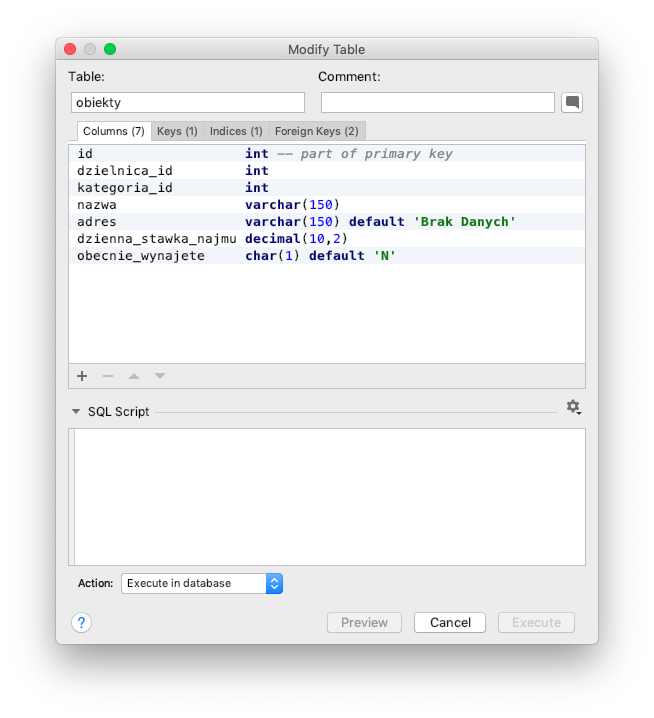
\includegraphics[width=0.4\textwidth]{objects}
	\caption{Tabela \texttt{obiekty} wyświetlona w programie \href{https://www.jetbrains.com/datagrip/}{DataGrip}}
	\label{fig:objects}
\end{figure}

\begin{lstlisting}[language=SQL, caption={Skrypt tworzący tabelę \texttt{obiekty}}, label={lst:table-objects}]
CREATE TABLE obiekty (
  id INT PRIMARY KEY NOT NULL IDENTITY (1, 1),

  dzielnica_id INT NOT NULL,
  kategoria_id INT NOT NULL,

  nazwa VARCHAR(150) NOT NULL,
  adres VARCHAR(150) NOT NULL DEFAULT 'Brak Danych',
  dzienna_stawka_najmu DECIMAL(10, 2) NOT NULL CHECK (dzienna_stawka_najmu > 0),

  obecnie_wynajete CHAR(1) NOT NULL DEFAULT 'N' CHECK (obecnie_wynajete IN ('T', 'N')),
);
\end{lstlisting}

\subsubsection{Utworzenie tabeli z najmami i utworzenie indeksu unikatowego w tabeli z najmami}

Przyjmujemy że domyślną datą rozpoczęcia najmu jest data jego dodania do bazy.

\begin{lstlisting}[language=SQL, caption={Skrypt tworzący tabelę \texttt{najmy}}, label={lst:table-najmy}]
CREATE TABLE najmy (
  id INT PRIMARY KEY NOT NULL IDENTITY (1, 1),

  uzytkownik_id INT NOT NULL,
  obiekt_id INT NOT NULL,

  data_rozpoczecia DATE NOT NULL DEFAULT getdate(),
  data_zakonczenia DATE NULL,
  koszt DECIMAL(15, 2) NULL,
);
\end{lstlisting}

\begin{figure}[h]
	\centering
    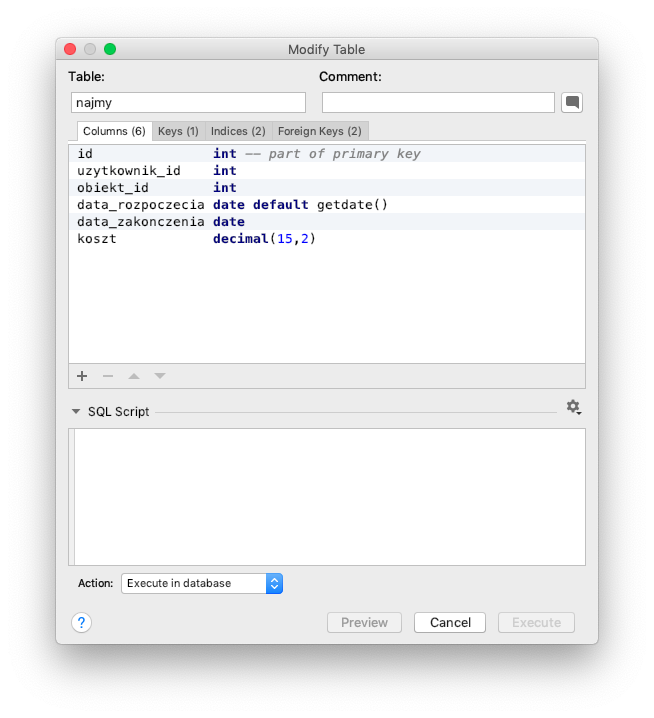
\includegraphics[width=0.4\textwidth]{najmy}
	\caption{Tabela \texttt{najmy} wyświetlona w programie \href{https://www.jetbrains.com/datagrip/}{DataGrip}}
	\label{fig:najmy}
\end{figure}

Ponieważ w założeniach projektowych przyjeliśmy że najem następuje od północy do godziny 23:59, to zostało wykorzystane pole typu \texttt{DATE}. Więc na przykład jeśli klient wynajmie dany obiekt tylko na jeden dzień to w polach \texttt{data\_rozpoczecia} oraz \texttt{data\_zakonczenia} wartość będzie ta sama. Dzięki temu możemy również utworzyć indeks unikatowy na pola \texttt{uzytkownik\_id}, \texttt{obiekt\_id} oraz \texttt{data\_rozpoczecia}.

\begin{lstlisting}[language=SQL, caption={Skrypt tworzący indeks unikatowy w tabeli \texttt{obiekty}}, label={lst:table-najmy}]
CREATE UNIQUE INDEX najemcy_ui
   ON najmy (uzytkownik_id, obiekt_id, data_rozpoczecia);
\end{lstlisting}

\subsubsection{Utworzenie relacji pomiędzy użytkownikami a najmami}

Wszystkie tabele zostały połączone relacją (`CONSTRAINT`) typu klucz obcy (`FOREIGN KEY`) tak jak na przykładzie z listingu \ref{lst:table-najmy-foreign}.

\begin{figure}[h]
	\centering
    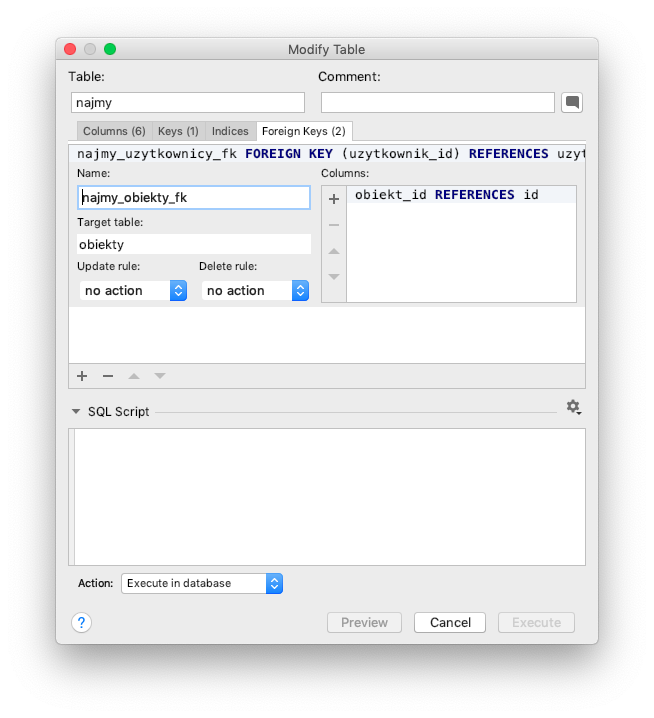
\includegraphics[width=0.4\textwidth]{najmy-foreign}
	\caption{Relacja \texttt{najmy\_obiekty\_fk} wyświetlona w programie \href{https://www.jetbrains.com/datagrip/}{DataGrip}}
	\label{fig:najmy-foreign}
\end{figure}

\begin{lstlisting}[language=SQL, caption={Skrypt tworzący relację \texttt{najmy\_obiekty\_fk}}, label={lst:table-najmy-foreign}]
ALTER TABLE najmy
  ADD CONSTRAINT najmy_obiekty_fk
  FOREIGN KEY (obiekt_id)
  REFERENCES obiekty(id);
\end{lstlisting}